\documentclass[11pt]{standalone}
\usepackage{amssymb}
\usepackage{amsmath}
\usepackage[no-math]{fontspec}
\usepackage{unicode-math}
\usepackage{libertinus}
\usepackage{pgf,xcolor}
\usepackage{tikz}
\usetikzlibrary{arrows.meta, backgrounds}
\usepackage{pgfplots}
\pgfplotsset{compat=newest}

% Additional packages
\usepackage{pgfplotsthemetol}  % not used, just pgfplots is enough

\definecolor{my_darkgray}{HTML}{484949}
\definecolor{my_lightgray}{HTML}{F3F4F4}
\definecolor{my_darkblue}{HTML}{005A94}
\definecolor{my_lightblue}{HTML}{CCDEE9}
\definecolor{my_yellow}{HTML}{FFEC7F}
\definecolor{my_red}{HTML}{E60000}
\definecolor{my_orange}{HTML}{E87846}

\begin{document}
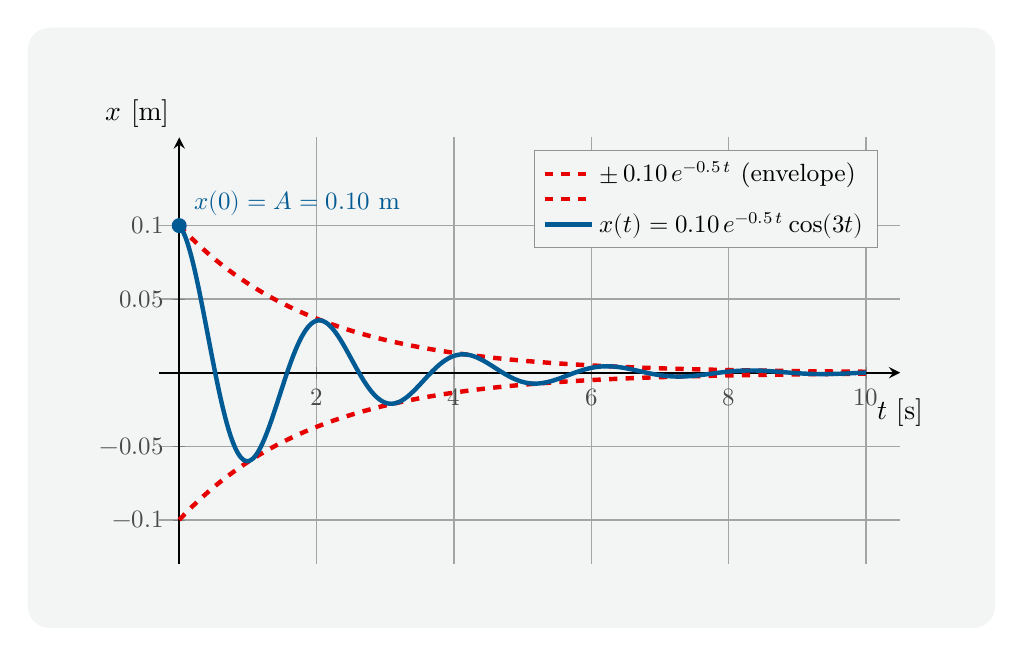
\begin{tikzpicture}[
    show background rectangle,
    background rectangle/.style={fill=my_lightgray, rounded corners=8pt},
    inner frame sep=0.8cm
]
\begin{axis}[
    axis lines = center,
    xlabel = {$t~[\text{s}]$},
    ylabel = {$x~[\text{m}]$},
    xlabel style = {at={(axis cs:10.5,0)}, anchor=north, yshift=-6pt},
    ylabel style = {anchor=south east},
    grid = both,
    grid style = {line width=0.3pt, draw=my_darkgray!30},
    major grid style = {line width=0.5pt, draw=my_darkgray!50},
    % axis equal omitted: x range ~0..10, y range ~-0.10..0.10
    % would make the graph unreadably flat at equal scaling
    axis line style = {thick},
    xmin = -0.3, xmax = 10.5,
    ymin = -0.13, ymax = 0.16,
    xtick = {0,2,4,6,8,10},
    ytick = {-0.10,-0.05,0,0.05,0.10},
    yticklabel style = {
        /pgf/number format/fixed,
        /pgf/number format/precision=2,
        font=\small,
        text=my_darkgray
    },
    xticklabel style = {font=\small, text=my_darkgray},
    width=11cm, height=7cm,
    legend pos=north east,
    legend style={font=\small, fill=my_lightgray, draw=my_darkgray!60},
    legend cell align=left,
    clip=false,
]

% Upper envelope: +0.10 * e^(-0.5t)
\addplot[
    draw=my_red,
    samples=300,
    ultra thick,
    dashed,
    domain=0:10
]{ 0.10 * exp(-0.5*x) };
\addlegendentry{$\pm\,0.10\,e^{-0.5\,t}$ (envelope)}

% Lower envelope: -0.10 * e^(-0.5t)
\addplot[
    draw=my_red,
    samples=300,
    ultra thick,
    dashed,
    domain=0:10
]{ -0.10 * exp(-0.5*x) };
\addlegendentry{}   % suppress duplicate legend entry

% Damped oscillation: x(t) = 0.10 * e^(-0.5t) * cos(3t)
\addplot[
    draw=my_darkblue,
    samples=600,
    ultra thick,
    domain=0:10
]{ 0.10 * exp(-0.5*x) * cos(deg(3*x)) };
\addlegendentry{$x(t)=0.10\,e^{-0.5\,t}\cos(3t)$}

% Mark the initial displacement x(0) = 0.10 m
\addplot[
    mark=*,
    mark size=2.5pt,
    only marks,
    draw=my_darkblue,
    fill=my_darkblue
] coordinates {(0, 0.10)};
\node[anchor=south west, font=\small, text=my_darkblue]
    at (axis cs:0.08, 0.10) {$x(0)=A=0.10~\text{m}$};

\end{axis}
\end{tikzpicture}
\end{document}
